\documentclass[12pt]{report}
\usepackage{titlesec}
\usepackage{lipsum}


\usepackage[a4paper, left=3.17cm, right=3.17cm, top=2.54cm, bottom=2.54cm]{geometry}
\usepackage[T1]{fontenc}

\usepackage{courier} %% Sets font for listing as Courier.
\usepackage{listings, xcolor}
\lstset{
tabsize = 4, %% set tab space width
showstringspaces = false, %% prevent space marking in strings, string is defined as the text that is generally printed directly to the console
numbers = left, %% display line numbers on the left
commentstyle = \color{green}, %% set comment color
keywordstyle = \color{blue}, %% set keyword color
stringstyle = \color{red}, %% set string color
rulecolor = \color{black}, %% set frame color to avoid being affected by text color
basicstyle = \small\ttfamily, %% set listing font and size
breaklines = true, %% enable line breaking
numberstyle = \tiny,
}
\usepackage{indentfirst}


\usepackage{mathptmx}
\usepackage{amsmath}
\usepackage{amsfonts}
\usepackage{chemformula}
\usepackage{multicol}
\usepackage{multirow}
\usepackage{tabularx,booktabs}
\newcolumntype{C}{>{\centering\arraybackslash}X} % centered version of "X" type
\usepackage[linesnumbered,ruled,vlined]{algorithm2e}
\usepackage{comment}
\usepackage{array}
\newcolumntype{P}[1]{>{\centering\arraybackslash}p{#1}}
\usepackage{cite}
\usepackage[colorlinks, linkcolor=black, anchorcolor=black, citecolor=black]{hyperref}
\usepackage{graphicx}
\usepackage{tikz}
\usetikzlibrary{shapes.geometric, arrows, positioning, fit, backgrounds, calc}

% Define styles for diagrams
\tikzstyle{startstop} = [rectangle, rounded corners, minimum width=3cm, minimum height=1cm, text centered, draw=black, fill=red!30]
\tikzstyle{process} = [rectangle, minimum width=3cm, minimum height=1cm, text centered, draw=black, fill=blue!20]
\tikzstyle{decision} = [diamond, minimum width=2.5cm, minimum height=1cm, text centered, draw=black, fill=green!20]
\tikzstyle{io} = [trapezium, trapezium left angle=70, trapezium right angle=110, minimum width=2.5cm, minimum height=1cm, text centered, draw=black, fill=orange!20]
\tikzstyle{arrow} = [thick,->,>=stealth]
\tikzstyle{layer} = [rectangle, rounded corners, minimum width=12cm, minimum height=1.5cm, text centered, draw=black, fill=blue!10]
\tikzstyle{component} = [rectangle, rounded corners, minimum width=2.5cm, minimum height=0.8cm, text centered, draw=black, fill=green!20]
\tikzstyle{database} = [cylinder, shape border rotate=90, draw, minimum height=1.5cm, minimum width=2cm, fill=yellow!20]

\setlength{\parskip}{0.5em}
\title{WhatsZ: WhatsApp Conversation Management Server}
%\author{\textup{Qi YUAN}}


%copyright at footer
\usepackage{fancyhdr}
\fancyhf{}
\rfoot{%
  \footnotesize
  \textcopyright~Dept. of Computer Science and Engineering, GUB\\

 }
%\pagestyle{fancy}


\begin{document}
    \input{title/title.tex}
   \tableofcontents
  
%

% Chapter 1 starting here.....    
\newpage
\chapter{Introduction}

\section{Overview}
\par This project focuses on the design and implementation of a WhatsApp Conversation Management Server that enables structured access to chat data through well-defined tools (APIs). The system is developed using the Zig programming language and follows a modular, tool-based architecture where each tool performs a specific operation related to WhatsApp chats, messages, and groups.

\par The server provides multiple functionalities such as listing all chats, retrieving messages from specific conversations, searching messages across chats, generating chat statistics, listing group conversations, and fetching group member information. Each functionality is registered as an independent tool using a standardized interface consisting of a tool name, description, and handler function. This approach improves code maintainability, scalability, and clarity.

\par The system implements the Model Context Protocol (MCP), which allows seamless integration with AI assistants like Claude, ChatGPT, and other LLM-based systems. By exposing WhatsApp data through MCP tools, AI models can dynamically query and analyze chat data based on user intent, enabling intelligent and efficient interaction with messaging history.

\par Overall, this project highlights practical backend development concepts such as API design, error handling, modular programming, database querying, and data retrieval, while also showcasing how modern messaging platforms can be integrated with intelligent systems for advanced analysis and automation.


\section{Motivation}
WhatsApp is one of the most widely used messaging platforms for personal and professional communication, generating a large amount of conversational data every day. This data has significant potential for automation, analysis, and AI-driven applications. However, accessing and managing WhatsApp conversation data in a structured and programmable way is challenging. This project is motivated by the need to design a modular backend server that can efficiently expose WhatsApp chats, messages, and group information for intelligent and automated systems.
\newline 
We were inspired to work on this project because:
\begin{itemize}
    \item Huge volume of WhatsApp chat data is generated daily
\item Lack of structured and programmable access to chat data
\item Existing systems are not automation-friendly
\item Need for modular and scalable backend architecture
\item Support for AI assistants and chatbot integration via MCP
\item Interest in exploring Zig as a systems programming language
    \end{itemize}
\section{Problem Definition}
Despite the popularity of WhatsApp, there is no standardized backend framework that allows developers to manage chats, messages, and groups programmatically. Chat data is often unstructured, making retrieval, searching, and analysis difficult. The project addresses this problem by proposing a tool-based WhatsApp management server that provides structured access to essential chat and group operations.
\begin{itemize}
    \item No unified backend system for WhatsApp data management
    \item Difficulty in retrieving messages from specific chats
    \item Inefficient message searching across conversations
    \item Lack of automated chat statistics generation
    \item Limited support for group and member management
    \item Poor integration with AI and automation workflows
    \item No existing MCP-compatible WhatsApp data interface
\end{itemize}
\newpage
\subsection{Complex Engineering Problem}


\begin{table}[htbp]

   \centering
    \caption{Summary of the attributes touched by this project}
    \begin{tabular}{|p{6.0 cm}|p{8 cm}|}
    %\rowcolor{gray!30}
    \toprule
        \textbf{Name of the Attributes} & \textbf{Explanation how to address}  \\
        \midrule

    \textbf{P1:} Depth of knowledge required  &  The project required knowledge of Zig programming, SQLite database operations, MCP protocol implementation, and understanding how WhatsApp stores data locally. Learning Zig's memory management and error handling was particularly challenging. \\
      \hline

    \textbf{P2:} Depth of analysis required  &  Analysis was needed to understand WhatsApp's SQLite schema, design efficient queries for chat retrieval, and implement pagination. Decisions included search functionality, timestamp conversion, and error handling strategies. \\
    \hline
    
    \textbf{P3:} Familiarity with issues  & Practical challenges such as handling Apple Core Data timestamps, large chat histories, partial name matching, database connection management, and cross-platform considerations were studied and addressed. \\ 
    \hline
    \textbf{P4:} Extent of applicable codes  &  Multiple handler functions were implemented for chat listing, message retrieval, searching, statistics generation, and group management. MCP protocol integration required proper registration and transport layer implementation. \\
      \hline
       
    \textbf{P5:} Extent of stakeholder
     involvement and conflicting
     requirements  & Different users and systems have varying expectations regarding performance, privacy, accuracy, and scalability. Privacy concerns with accessing local WhatsApp data were considered in the design. \\
      \hline

    \textbf{P6:} Interdependence  &  The components are highly interdependent. The MCP server, SQLite database layer, and tool handlers must work together seamlessly. A failure in database connection affects all tools. \\
    \hline
        
    \end{tabular}
    \label{tab:CEP}
\end{table}

\newpage
\section{Design Objectives}
The main objectives of this project are: 
\begin{itemize}
    \item To design a modular tool-based backend server in Zig
    \item To enable structured access to WhatsApp chats, messages, and groups
    \item To implement MCP (Model Context Protocol) for AI assistant integration
    \item To implement error-safe API registration using Zig's error handling
    \item To support efficient querying with pagination and search capabilities
   
\end{itemize}

\section{Application}
The proposed system can be applied in several real-life scenarios, including:
\begin{itemize}
    \item \textbf{AI chatbots and virtual assistants} – to access and respond to user chats efficiently via MCP integration with Claude, ChatGPT, etc.
    \item \textbf{Personal productivity tools} – for searching and organizing chat history intelligently.
    \item \textbf{Team collaboration analysis} – for analyzing group chats and tracking communication patterns.
    \item \textbf{Data analysis and research} – for studying messaging behavior, trends, and chat-based statistics.
     \item \textbf{Automation systems} – to integrate WhatsApp data with workflow automation and notification systems.
    
\end{itemize}

\begin{figure}[htbp]
\centering
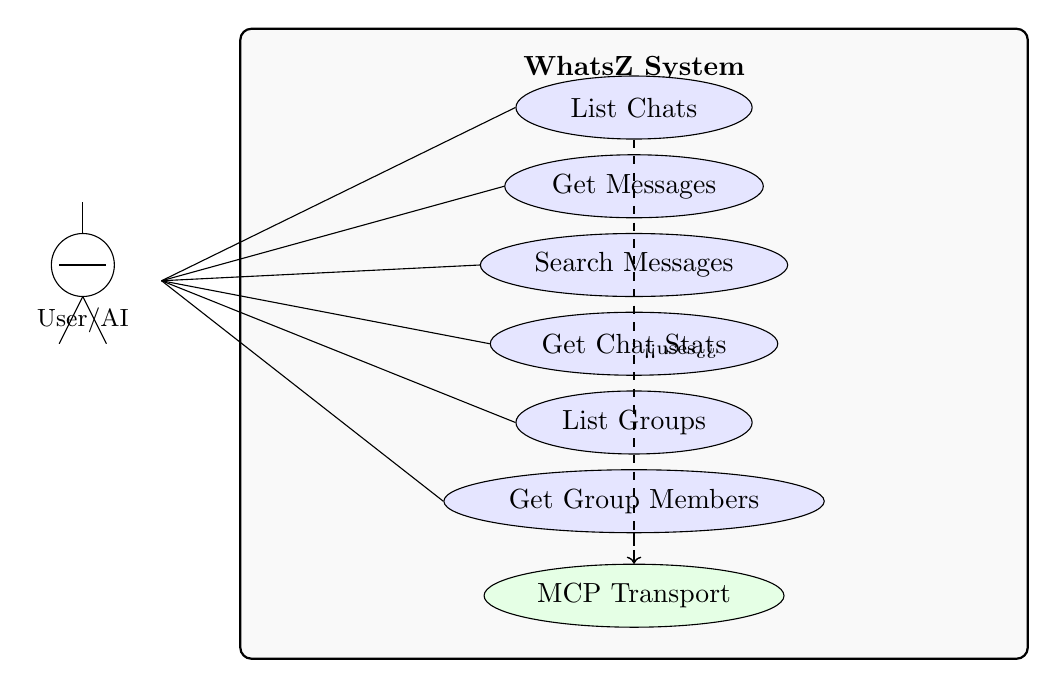
\begin{tikzpicture}[node distance=0.6cm]
    % System boundary
    \draw [rounded corners, thick, fill=gray!5] (-1,-5) rectangle (9,3);
    \node at (4,2.5) [font=\bfseries] {WhatsZ System};
    
    % Actor
    \node (user) at (-3,0) [circle, draw, minimum size=0.8cm] {};
    \node at (-3,-0.7) [font=\small] {User/AI};
    \draw (-3,0.4) -- (-3,0.8);
    \draw (-3.3,0) -- (-2.7,0);
    \draw (-3,-0.4) -- (-3.3,-1);
    \draw (-3,-0.4) -- (-2.7,-1);
    
    % Use cases
    \node (uc1) [ellipse, draw, fill=blue!10, minimum width=3cm, minimum height=0.8cm] at (4,2) {List Chats};
    \node (uc2) [ellipse, draw, fill=blue!10, minimum width=3cm, minimum height=0.8cm] at (4,1) {Get Messages};
    \node (uc3) [ellipse, draw, fill=blue!10, minimum width=3cm, minimum height=0.8cm] at (4,0) {Search Messages};
    \node (uc4) [ellipse, draw, fill=blue!10, minimum width=3cm, minimum height=0.8cm] at (4,-1) {Get Chat Stats};
    \node (uc5) [ellipse, draw, fill=blue!10, minimum width=3cm, minimum height=0.8cm] at (4,-2) {List Groups};
    \node (uc6) [ellipse, draw, fill=blue!10, minimum width=3cm, minimum height=0.8cm] at (4,-3) {Get Group Members};
    \node (uc7) [ellipse, draw, fill=green!10, minimum width=3cm, minimum height=0.8cm] at (4,-4.2) {MCP Transport};
    
    % Connections
    \draw [-] (-2,-0.2) -- (uc1.west);
    \draw [-] (-2,-0.2) -- (uc2.west);
    \draw [-] (-2,-0.2) -- (uc3.west);
    \draw [-] (-2,-0.2) -- (uc4.west);
    \draw [-] (-2,-0.2) -- (uc5.west);
    \draw [-] (-2,-0.2) -- (uc6.west);
    
    % Include relationship
    \draw [dashed, ->] (uc1) -- node[right, font=\scriptsize] {<<uses>>} (uc7);
    \draw [dashed, ->] (uc6) -- (uc7);
\end{tikzpicture}
\caption{Use Case Diagram for WhatsZ}
\label{fig:usecase}
\end{figure}


% Chapter 1 ends here.....    




% Chapter 2 starting here.....    
\newpage
\chapter{Design/Development/Implementation of the Project}

\section{Introduction}
\par Instant messaging applications like WhatsApp have become an integral part of personal and professional communication. With billions of messages exchanged daily, a large amount of conversational data is generated, containing valuable information that can be used for analysis, automation, and AI-driven applications. However, accessing and managing this data in a structured and programmable way is challenging, as existing solutions are often manual, unstructured, or platform-dependent.

\par This project proposes a WhatsApp Conversation Management Server that provides structured access to chats, messages, and group information through modular, tool-based APIs implementing the Model Context Protocol (MCP). The server is implemented using the Zig programming language and follows a clean architecture where each tool performs a specific task, such as listing chats, retrieving messages, searching conversations, generating chat statistics, or managing group members.

\par The system is designed to be scalable, reliable, and easily integrable with AI assistants, chatbots, and automation systems through the MCP standard, making it suitable for both practical applications and development workflows. By enabling structured access to WhatsApp data, this project demonstrates how messaging platforms can be leveraged for intelligent data analysis and automation workflows.

\section{Project Details}
\subsection{Language and Technology Choices:}
\begin{itemize}
    \item \textbf{Zig Programming Language} – chosen for its performance, memory safety, and compile-time features. Zig provides explicit error handling and zero-cost abstractions.
    \item \textbf{SQLite} – WhatsApp stores chat data locally in SQLite format. The project uses zqlite (Zig SQLite bindings) for database operations.
    \item \textbf{MCP (Model Context Protocol)} – an open protocol for AI assistant integration, allowing tools to be exposed and called by AI models.
    \item \textbf{ZX Framework} – used for the web interface component of the project.
\end{itemize}

\subsection{Design Choices:}
\begin{itemize}
    \item \textbf{Tool-based Architecture} – Each functionality is registered as an independent tool with a name, description, and handler function, promoting modularity.
    \item \textbf{Read-only Database Access} – The system opens WhatsApp's database in read-only mode to ensure data integrity and safety.
    \item \textbf{STDIO Transport} – MCP communication uses STDIO transport for compatibility with various AI assistant integrations.
    \item \textbf{Pagination Support} – All list operations support limit and offset parameters for handling large datasets.
\end{itemize}

\subsection{Component Diagram}
The following diagram shows the major components of the WhatsZ system and their dependencies:

\begin{figure}[htbp]
\centering
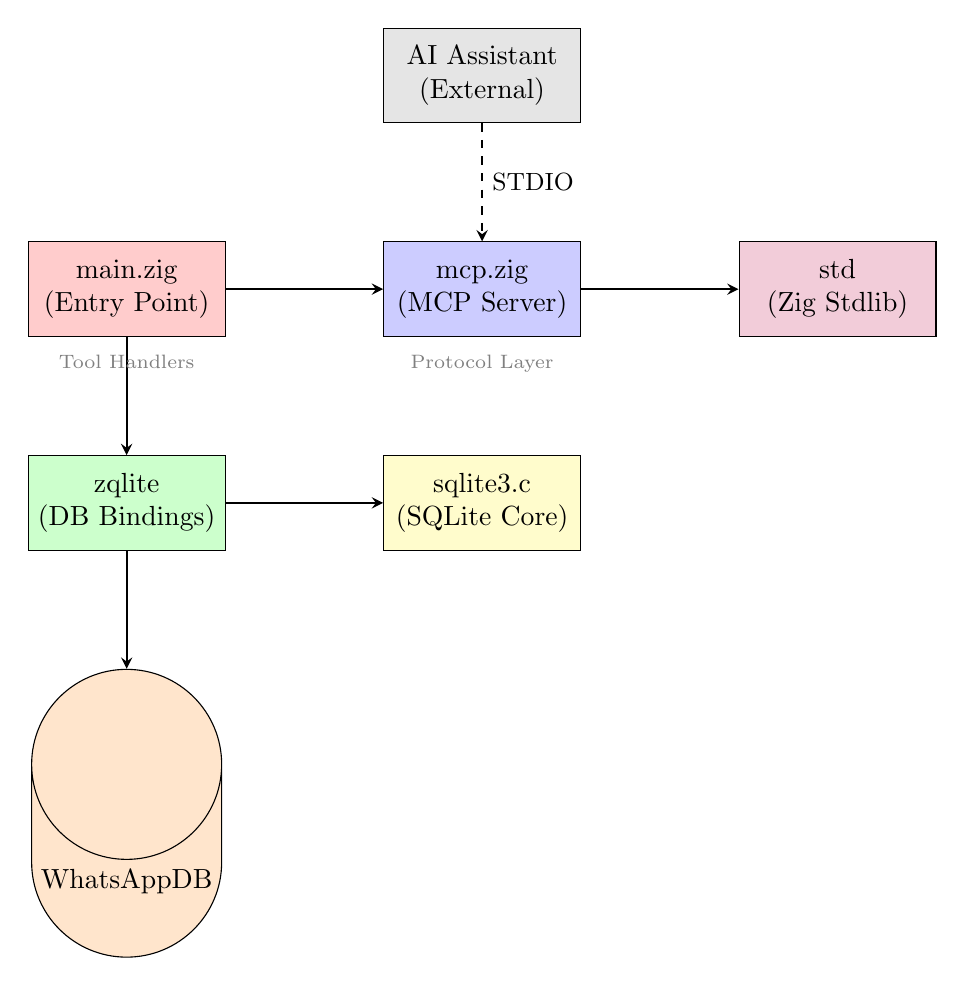
\begin{tikzpicture}[node distance=1cm]
    % Main components
    \node (main) [rectangle, draw, fill=red!20, minimum width=2.5cm, minimum height=1.2cm, align=center] {main.zig\\(Entry Point)};
    
    \node (mcp) [rectangle, draw, fill=blue!20, minimum width=2.5cm, minimum height=1.2cm, align=center, right=2cm of main] {mcp.zig\\(MCP Server)};
    
    \node (zqlite) [rectangle, draw, fill=green!20, minimum width=2.5cm, minimum height=1.2cm, align=center, below=1.5cm of main] {zqlite\\(DB Bindings)};
    
    \node (sqlite) [rectangle, draw, fill=yellow!20, minimum width=2.5cm, minimum height=1.2cm, align=center, below=1.5cm of mcp] {sqlite3.c\\(SQLite Core)};
    
    \node (std) [rectangle, draw, fill=purple!20, minimum width=2.5cm, minimum height=1.2cm, align=center, right=2cm of mcp] {std\\(Zig Stdlib)};
    
    % External
    \node (wa) [cylinder, shape border rotate=90, draw, fill=orange!20, minimum height=1cm, minimum width=1.5cm, below=1.5cm of zqlite] {WhatsApp\\DB};
    
    \node (ai) [rectangle, draw, fill=gray!20, minimum width=2.5cm, minimum height=1.2cm, align=center, above=1.5cm of mcp] {AI Assistant\\(External)};
    
    % Dependencies
    \draw [arrow] (main) -- (mcp);
    \draw [arrow] (main) -- (zqlite);
    \draw [arrow] (mcp) -- (std);
    \draw [arrow] (zqlite) -- (sqlite);
    \draw [arrow] (zqlite) -- (wa);
    \draw [arrow, dashed] (ai) -- node[right, font=\small] {STDIO} (mcp);
    
    % Labels
    \node [below=0.1cm of main, font=\scriptsize, text=gray] {Tool Handlers};
    \node [below=0.1cm of mcp, font=\scriptsize, text=gray] {Protocol Layer};
\end{tikzpicture}
\caption{Component Dependency Diagram}
\label{fig:components}
\end{figure}

\section{Implementation}

\subsection{System Architecture}
The system follows a layered architecture consisting of:

\begin{itemize}
    \item \textbf{MCP Server Layer} – Handles protocol communication, tool registration, and request routing.
    \item \textbf{Tool Handler Layer} – Contains individual handler functions for each tool (list\_chats, get\_chat\_messages, etc.).
    \item \textbf{Database Layer} – Manages SQLite connections and query execution using zqlite bindings.
    \item \textbf{Utility Layer} – Provides helper functions like timestamp conversion and string building.
\end{itemize}

\begin{figure}[htbp]
\centering
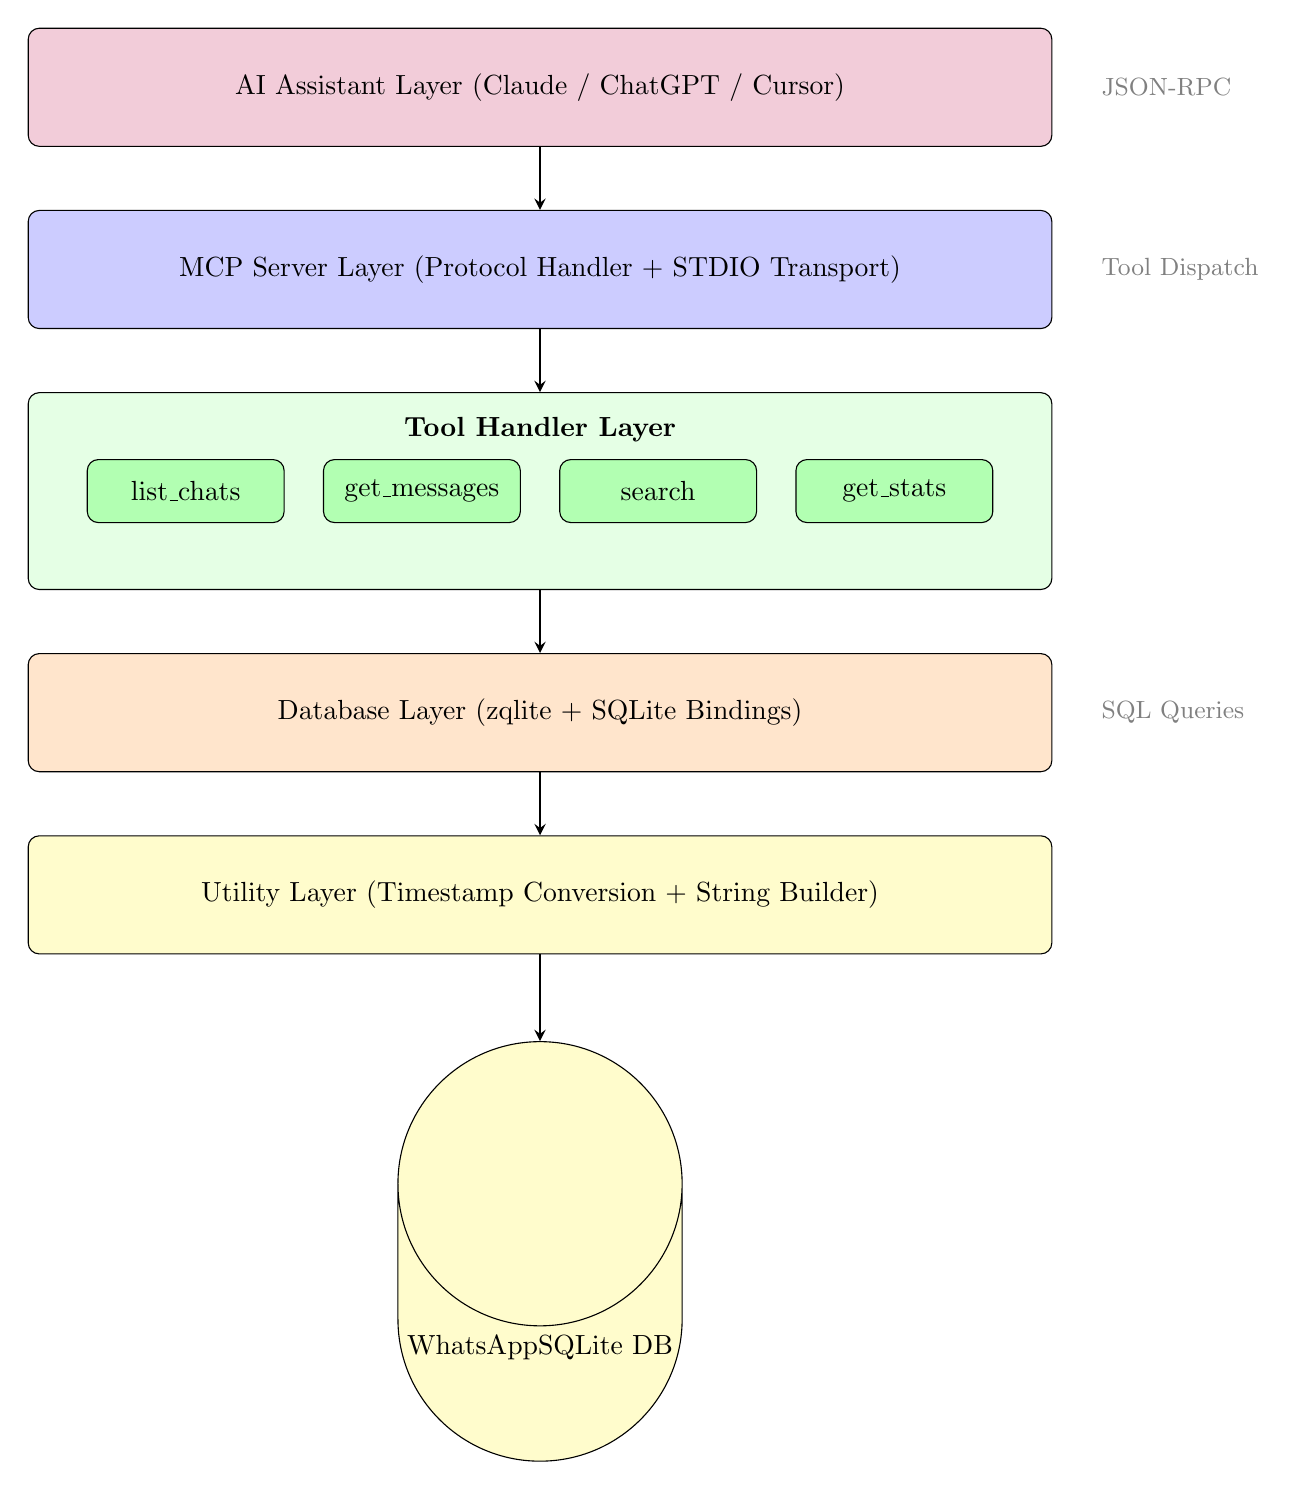
\begin{tikzpicture}[node distance=0.8cm]
    % AI Layer
    \node (ai) [layer, fill=purple!20, minimum width=13cm] {AI Assistant Layer (Claude / ChatGPT / Cursor)};
    
    % MCP Server Layer
    \node (mcp) [layer, fill=blue!20, below=of ai, minimum width=13cm] {MCP Server Layer (Protocol Handler + STDIO Transport)};
    
    % Tool Handler Layer with individual tools
    \node (tools) [layer, fill=green!10, below=of mcp, minimum width=13cm, minimum height=2.5cm] {};
    \node at (tools.north) [anchor=north, yshift=-0.2cm] {\textbf{Tool Handler Layer}};
    
    % Individual tool boxes
    \node (t1) [component, fill=green!30] at ($(tools.center)+(-4.5,0)$) {list\_chats};
    \node (t2) [component, fill=green!30] at ($(tools.center)+(-1.5,0)$) {get\_messages};
    \node (t3) [component, fill=green!30] at ($(tools.center)+(1.5,0)$) {search};
    \node (t4) [component, fill=green!30] at ($(tools.center)+(4.5,0)$) {get\_stats};
    
    % Database Layer
    \node (db) [layer, fill=orange!20, below=of tools, minimum width=13cm] {Database Layer (zqlite + SQLite Bindings)};
    
    % Utility Layer
    \node (util) [layer, fill=yellow!20, below=of db, minimum width=13cm] {Utility Layer (Timestamp Conversion + String Builder)};
    
    % WhatsApp Database
    \node (wadb) [database, below=of util, yshift=-0.3cm, minimum width=3cm] {WhatsApp\\SQLite DB};
    
    % Arrows
    \draw [arrow] (ai) -- (mcp);
    \draw [arrow] (mcp) -- (tools);
    \draw [arrow] (tools) -- (db);
    \draw [arrow] (db) -- (util);
    \draw [arrow] (util) -- (wadb);
    
    % Labels
    \node [right=0.5cm of ai, text=gray] {\small JSON-RPC};
    \node [right=0.5cm of mcp, text=gray] {\small Tool Dispatch};
    \node [right=0.5cm of db, text=gray] {\small SQL Queries};
\end{tikzpicture}
\caption{WhatsZ System Architecture Diagram}
\label{fig:architecture}
\end{figure}

\subsection{Implemented Tools}
The following tools are implemented in the system:

\begin{enumerate}
    \item \textbf{list\_chats} – Lists all WhatsApp chats/conversations with name, last message, unread count, and last activity date.
    \item \textbf{get\_chat\_messages} – Retrieves messages from a specific chat using partial name matching or exact JID, with pagination support.
    \item \textbf{search\_messages} – Searches for messages containing specific text across all chats.
    \item \textbf{get\_chat\_stats} – Generates statistics for a chat including message count, date range, and media counts.
    \item \textbf{list\_groups} – Lists all WhatsApp group chats with member count and creation info.
    \item \textbf{get\_group\_members} – Retrieves members of a specific group with admin status and activity state.
\end{enumerate}

\subsection{Data Flow Diagram}
The following diagram illustrates how data flows through the WhatsZ system from user request to response:

\begin{figure}[htbp]
\centering
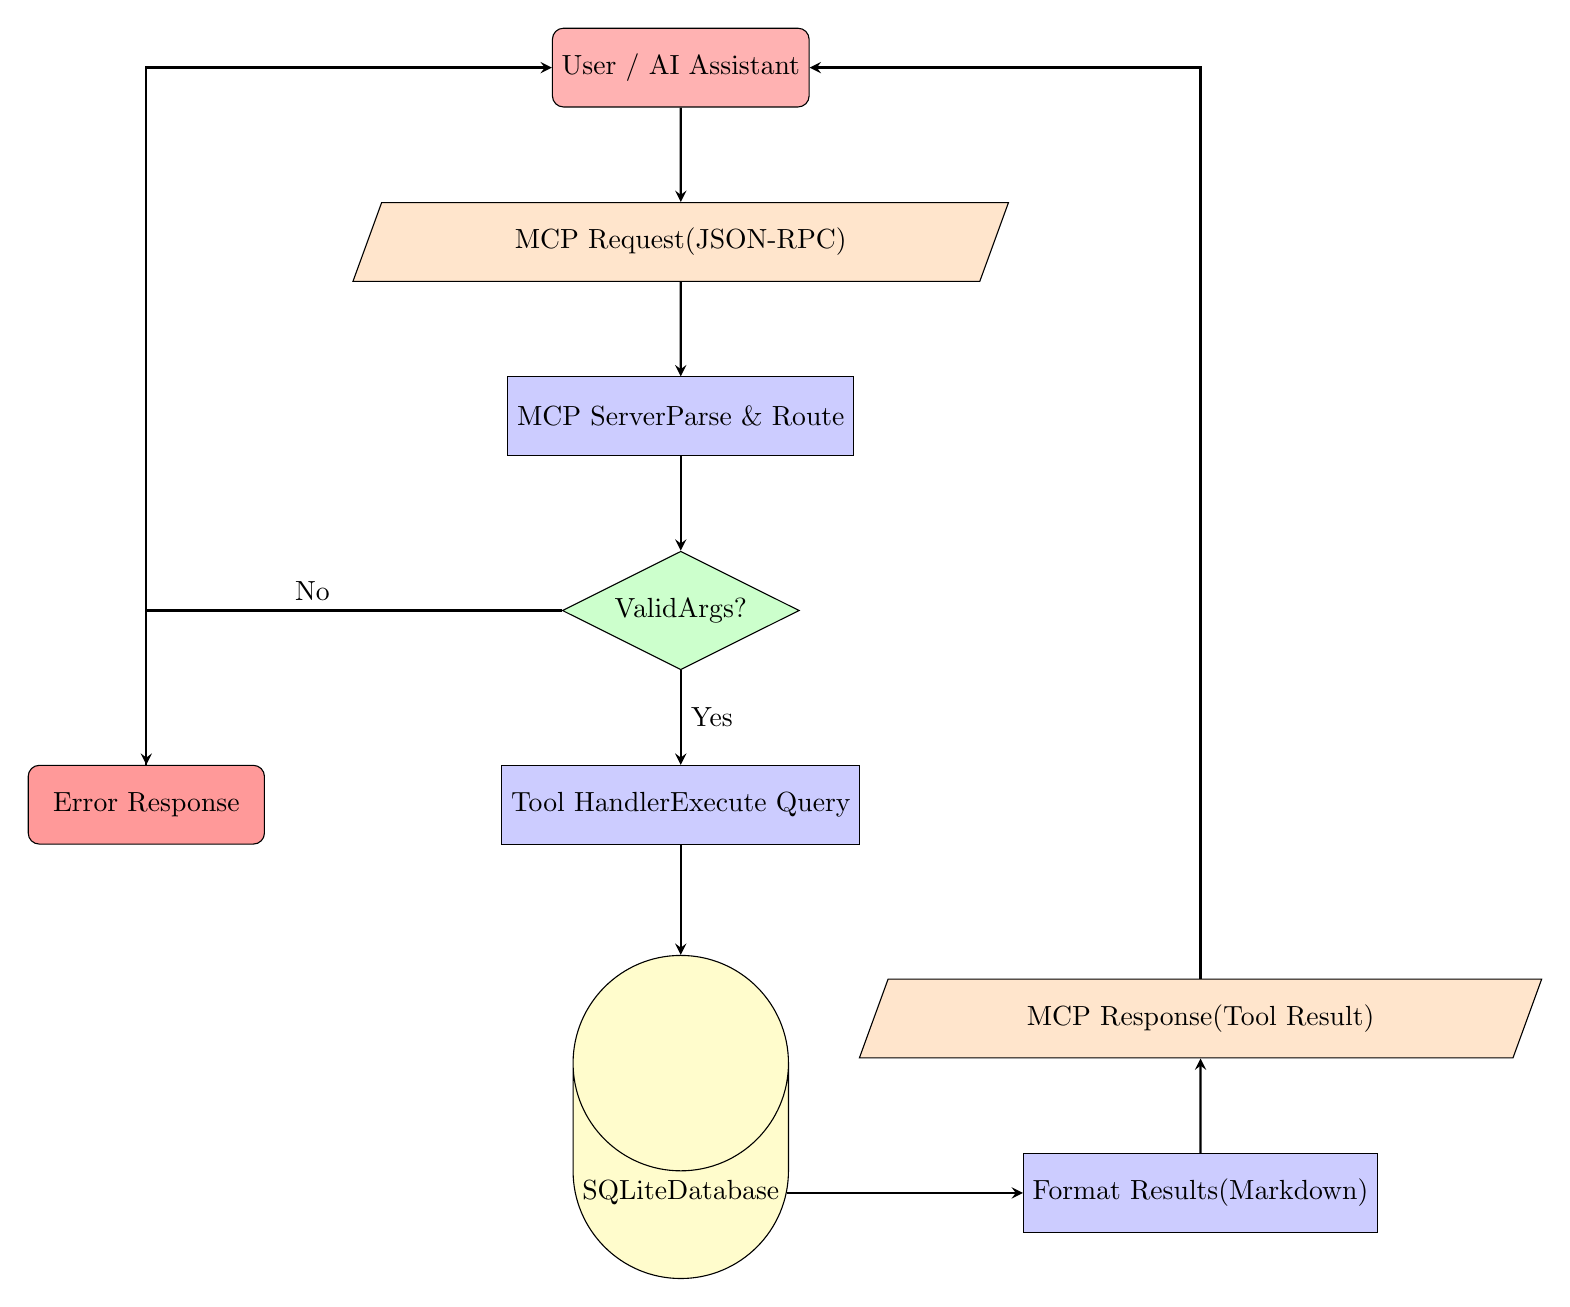
\begin{tikzpicture}[node distance=1.2cm]
    % Nodes
    \node (user) [startstop] {User / AI Assistant};
    \node (request) [io, below=of user] {MCP Request\\(JSON-RPC)};
    \node (server) [process, below=of request] {MCP Server\\Parse \& Route};
    \node (validate) [decision, below=of server, aspect=2] {Valid\\Args?};
    \node (handler) [process, below=of validate] {Tool Handler\\Execute Query};
    \node (db) [database, below=of handler, yshift=-0.2cm] {SQLite\\Database};
    \node (format) [process, right=3cm of db] {Format Results\\(Markdown)};
    \node (response) [io, above=of format] {MCP Response\\(Tool Result)};
    \node (error) [startstop, left=3cm of handler, fill=red!40] {Error Response};
    
    % Arrows
    \draw [arrow] (user) -- (request);
    \draw [arrow] (request) -- (server);
    \draw [arrow] (server) -- (validate);
    \draw [arrow] (validate) -- node[anchor=west] {Yes} (handler);
    \draw [arrow] (validate) -| node[anchor=south, pos=0.3] {No} (error);
    \draw [arrow] (handler) -- (db);
    \draw [arrow] (db) -- (format);
    \draw [arrow] (format) -- (response);
    \draw [arrow] (response) |- (user);
    \draw [arrow] (error) |- (user);
\end{tikzpicture}
\caption{Data Flow Diagram for WhatsZ Request Processing}
\label{fig:dataflow}
\end{figure}


\subsection{Tools and Libraries}
    \begin{itemize}
        \item \textbf{Zig 0.13+}: Primary programming language for the server implementation.
        \item \textbf{zqlite}: Zig bindings for SQLite database operations.
        \item \textbf{mcp.zig}: MCP protocol implementation library for Zig.
        \item \textbf{ZX}: Web framework for the site component.
        \item \textbf{SQLite3}: Embedded database engine for reading WhatsApp data.
    \end{itemize}

\subsection{Database Schema Diagram}
The WhatsZ system interacts with WhatsApp's local SQLite database, which contains the following key tables:

\begin{figure}[htbp]
\centering
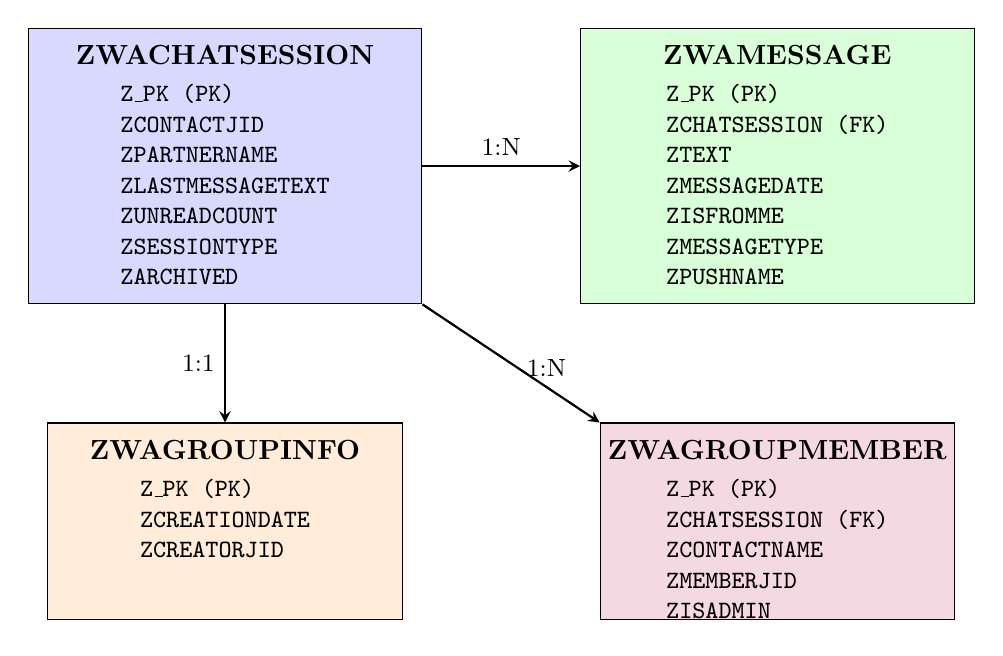
\begin{tikzpicture}[node distance=0.5cm]
    % Chat Session Table
    \node (chat) [rectangle, draw, fill=blue!15, minimum width=5cm, minimum height=3.5cm] {};
    \node at (chat.north) [anchor=north, yshift=-0.1cm, font=\bfseries] {ZWACHATSESSION};
    \node at (chat.north) [anchor=north, yshift=-0.6cm, align=left, font=\small\ttfamily] {
        Z\_PK (PK)\\
        ZCONTACTJID\\
        ZPARTNERNAME\\
        ZLASTMESSAGETEXT\\
        ZUNREADCOUNT\\
        ZSESSIONTYPE\\
        ZARCHIVED
    };
    
    % Message Table
    \node (msg) [rectangle, draw, fill=green!15, minimum width=5cm, minimum height=3.5cm, right=2cm of chat] {};
    \node at (msg.north) [anchor=north, yshift=-0.1cm, font=\bfseries] {ZWAMESSAGE};
    \node at (msg.north) [anchor=north, yshift=-0.6cm, align=left, font=\small\ttfamily] {
        Z\_PK (PK)\\
        ZCHATSESSION (FK)\\
        ZTEXT\\
        ZMESSAGEDATE\\
        ZISFROMME\\
        ZMESSAGETYPE\\
        ZPUSHNAME
    };
    
    % Group Info Table
    \node (group) [rectangle, draw, fill=orange!15, minimum width=4.5cm, minimum height=2.5cm, below=1.5cm of chat] {};
    \node at (group.north) [anchor=north, yshift=-0.1cm, font=\bfseries] {ZWAGROUPINFO};
    \node at (group.north) [anchor=north, yshift=-0.6cm, align=left, font=\small\ttfamily] {
        Z\_PK (PK)\\
        ZCREATIONDATE\\
        ZCREATORJID
    };
    
    % Group Member Table
    \node (member) [rectangle, draw, fill=purple!15, minimum width=4.5cm, minimum height=2.5cm, below=1.5cm of msg] {};
    \node at (member.north) [anchor=north, yshift=-0.1cm, font=\bfseries] {ZWAGROUPMEMBER};
    \node at (member.north) [anchor=north, yshift=-0.6cm, align=left, font=\small\ttfamily] {
        Z\_PK (PK)\\
        ZCHATSESSION (FK)\\
        ZCONTACTNAME\\
        ZMEMBERJID\\
        ZISADMIN
    };
    
    % Relationships
    \draw [arrow] (chat.east) -- node[above, font=\small] {1:N} (msg.west);
    \draw [arrow] (chat.south) -- node[left, font=\small] {1:1} (group.north);
    \draw [arrow] (chat.south east) -- node[above, font=\small, pos=0.7] {1:N} (member.north west);
\end{tikzpicture}
\caption{WhatsApp SQLite Database Schema (Key Tables)}
\label{fig:schema}
\end{figure}



\section{Implementation Details}

\subsection{Server Initialization}
\begin{enumerate}
    \item Initialize general purpose allocator for memory management.
    \item Create MCP server instance with name and version.
    \item Register all tool handlers with the server.
    \item Start server with STDIO transport for AI assistant communication.
\end{enumerate}

\subsection{Database Operations}
\begin{enumerate}
    \item Open WhatsApp SQLite database in read-only mode.
    \item Execute parameterized SQL queries to prevent injection.
    \item Process result rows and format output as Markdown.
    \item Handle Apple Core Data timestamps by converting to Unix time.
\end{enumerate}

\subsection{Tool Handler Flow}
\begin{enumerate}
    \item Parse input arguments from JSON payload.
    \item Validate required parameters and return errors if missing.
    \item Execute database queries with provided parameters.
    \item Format results as human-readable Markdown text.
    \item Return tool result with content for MCP response.
\end{enumerate}

\begin{figure}[htbp]
\centering
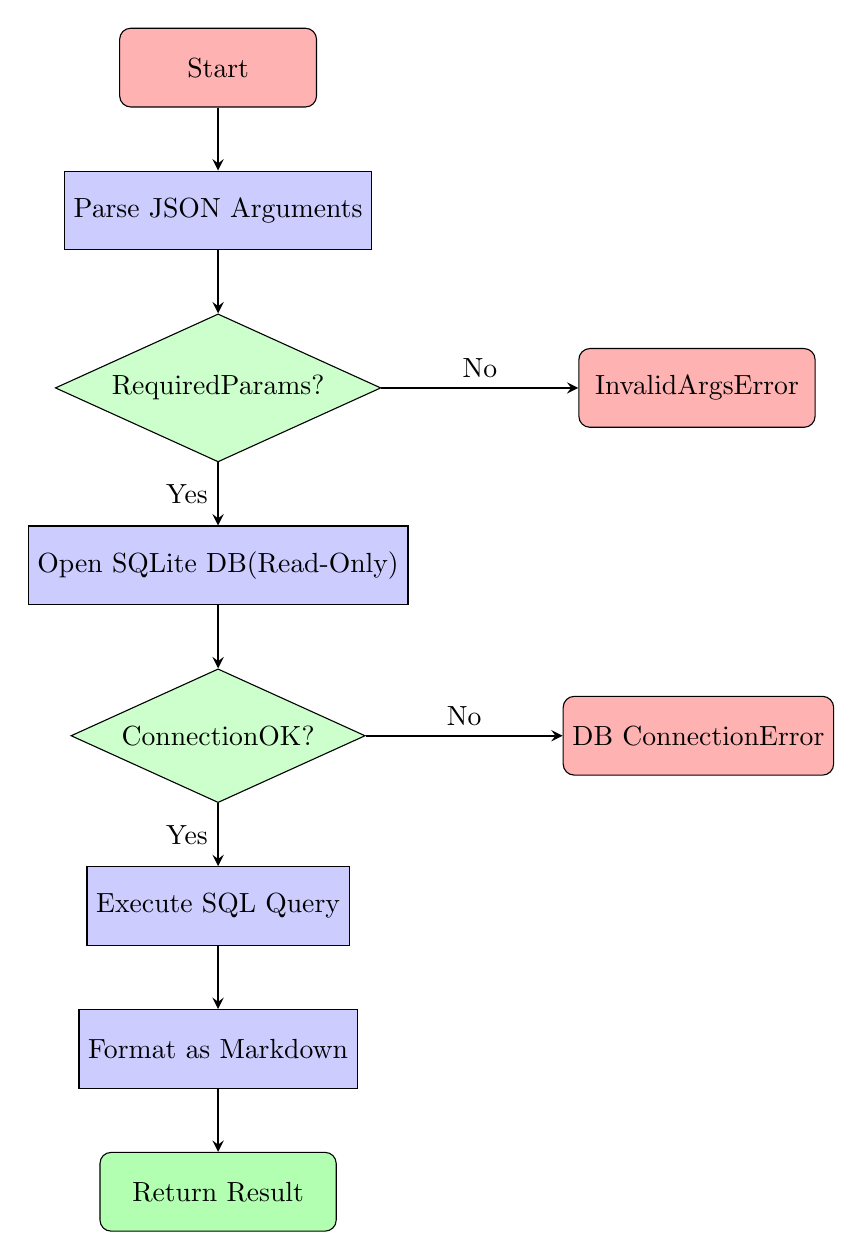
\begin{tikzpicture}[node distance=0.8cm]
    % Start
    \node (start) [startstop, minimum width=2.5cm] {Start};
    
    % Parse Args
    \node (parse) [process, below=of start] {Parse JSON Arguments};
    
    % Validate
    \node (validate) [decision, below=of parse, aspect=2.2] {Required\\Params?};
    
    % Open DB
    \node (opendb) [process, below=of validate] {Open SQLite DB\\(Read-Only)};
    
    % DB Check
    \node (dbcheck) [decision, below=of opendb, aspect=2.2] {Connection\\OK?};
    
    % Execute Query
    \node (query) [process, below=of dbcheck] {Execute SQL Query};
    
    % Format
    \node (format) [process, below=of query] {Format as Markdown};
    
    % Return Success
    \node (success) [startstop, below=of format, fill=green!30] {Return Result};
    
    % Error nodes
    \node (err1) [startstop, right=2.5cm of validate, fill=red!30] {InvalidArgs\\Error};
    \node (err2) [startstop, right=2.5cm of dbcheck, fill=red!30] {DB Connection\\Error};
    
    % Arrows
    \draw [arrow] (start) -- (parse);
    \draw [arrow] (parse) -- (validate);
    \draw [arrow] (validate) -- node[anchor=east] {Yes} (opendb);
    \draw [arrow] (validate) -- node[anchor=south] {No} (err1);
    \draw [arrow] (opendb) -- (dbcheck);
    \draw [arrow] (dbcheck) -- node[anchor=east] {Yes} (query);
    \draw [arrow] (dbcheck) -- node[anchor=south] {No} (err2);
    \draw [arrow] (query) -- (format);
    \draw [arrow] (format) -- (success);
\end{tikzpicture}
\caption{Tool Handler Execution Flowchart}
\label{fig:toolflow}
\end{figure}

\subsection{Error Handling}
\begin{enumerate}
    \item Database connection failures return descriptive error messages.
    \item Missing required parameters return InvalidArguments error.
    \item Query failures are caught and reported gracefully.
    \item Resource not found errors are handled for missing chats/groups.
\end{enumerate}

\subsection{MCP Protocol Communication}
The following sequence diagram illustrates how the MCP protocol enables communication between AI assistants and the WhatsZ server:

\begin{figure}[htbp]
\centering
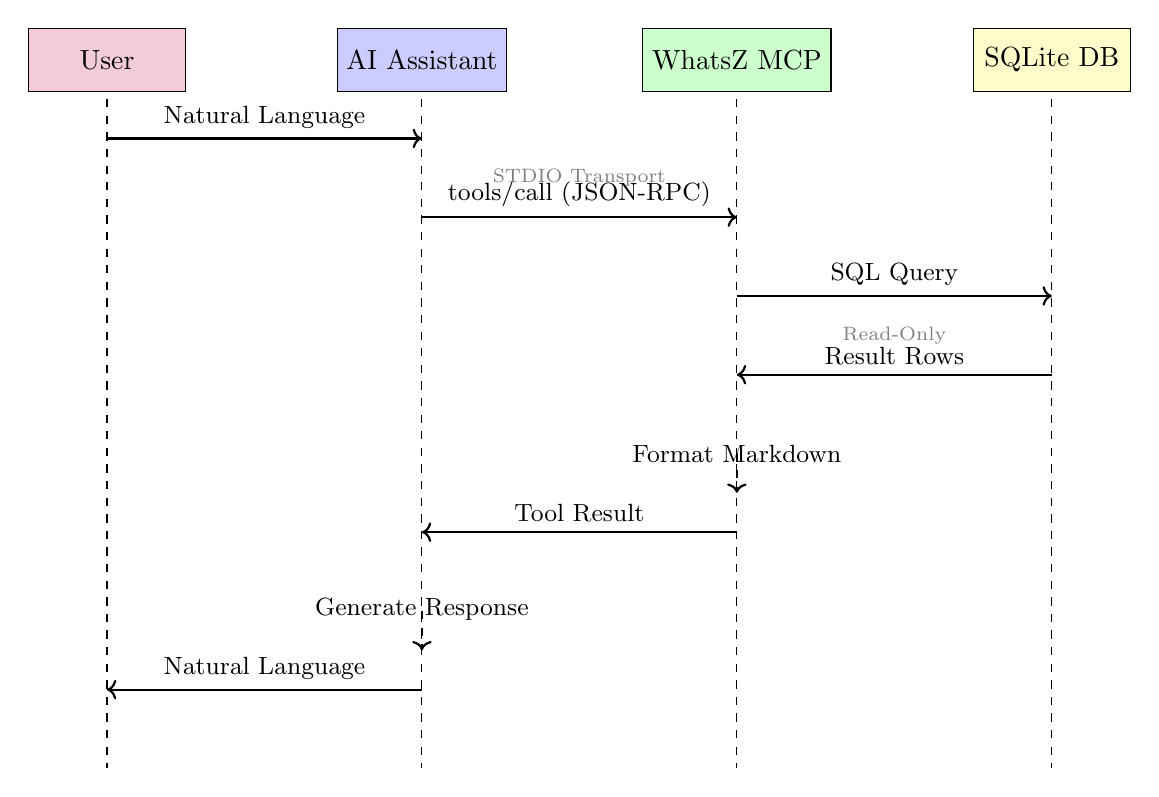
\begin{tikzpicture}
    % Actors
    \node (user) at (0,0) [rectangle, draw, fill=purple!20, minimum width=2cm, minimum height=0.8cm] {User};
    \node (ai) at (4,0) [rectangle, draw, fill=blue!20, minimum width=2cm, minimum height=0.8cm] {AI Assistant};
    \node (mcp) at (8,0) [rectangle, draw, fill=green!20, minimum width=2cm, minimum height=0.8cm] {WhatsZ MCP};
    \node (db) at (12,0) [rectangle, draw, fill=yellow!20, minimum width=2cm, minimum height=0.8cm] {SQLite DB};
    
    % Lifelines
    \draw [dashed] (0,-0.5) -- (0,-9);
    \draw [dashed] (4,-0.5) -- (4,-9);
    \draw [dashed] (8,-0.5) -- (8,-9);
    \draw [dashed] (12,-0.5) -- (12,-9);
    
    % Messages
    \draw [->, thick] (0,-1) -- node[above, font=\small] {Natural Language} (4,-1);
    \draw [->, thick] (4,-2) -- node[above, font=\small] {tools/call (JSON-RPC)} (8,-2);
    \draw [->, thick] (8,-3) -- node[above, font=\small] {SQL Query} (12,-3);
    \draw [<-, thick] (8,-4) -- node[above, font=\small] {Result Rows} (12,-4);
    \draw [->, thick, dashed] (8,-5) -- node[above, font=\small] {Format Markdown} (8,-5.5);
    \draw [<-, thick] (4,-6) -- node[above, font=\small] {Tool Result} (8,-6);
    \draw [->, thick, dashed] (4,-7) -- node[above, font=\small] {Generate Response} (4,-7.5);
    \draw [<-, thick] (0,-8) -- node[above, font=\small] {Natural Language} (4,-8);
    
    % Labels
    \node at (6,-1.5) [font=\scriptsize, text=gray] {STDIO Transport};
    \node at (10,-3.5) [font=\scriptsize, text=gray] {Read-Only};
\end{tikzpicture}
\caption{MCP Protocol Communication Sequence}
\label{fig:sequence}
\end{figure}



% Chapter 3 ends here..... 








% Chapter 4 starting here..... 
\newpage
\chapter{Performance Evaluation}

\section{Development Environment}
The development and testing environment for \textbf{WhatsZ} was set up on macOS with the following specifications:
\begin{itemize}
    \item \textbf{Operating System:} macOS (Darwin)
    \item \textbf{Compiler:} Zig 0.13+
    \item \textbf{Database:} SQLite 3.x (embedded)
    \item \textbf{WhatsApp Data:} Local ChatStorage.sqlite from WhatsApp Desktop
    \item \textbf{MCP Client:} Claude Desktop, Cursor IDE
\end{itemize}

\section{Functional Testing Results}
The system was tested with real WhatsApp chat data to verify all tools function correctly:

\begin{table}[htbp]
\centering
\caption{Functional Test Results}
\begin{tabular}{|p{4cm}|p{6cm}|p{3cm}|}
\toprule
\textbf{Tool} & \textbf{Test Case} & \textbf{Result} \\
\midrule
list\_chats & List 20 recent chats & Pass \\
\hline
get\_chat\_messages & Retrieve messages by name & Pass \\
\hline
get\_chat\_messages & Retrieve messages by JID & Pass \\
\hline
search\_messages & Search for keyword & Pass \\
\hline
get\_chat\_stats & Get statistics for chat & Pass \\
\hline
list\_groups & List all groups & Pass \\
\hline
get\_group\_members & Get members of group & Pass \\
\hline
Error Handling & Invalid parameters & Pass \\
\hline
Pagination & Limit and offset & Pass \\
\bottomrule
\end{tabular}
\label{tab:test_results}
\end{table}

\section{Results Analysis}
\begin{itemize}
    \item \textbf{Chat Listing:} Successfully retrieves all chats with proper ordering by last message date.
    \item \textbf{Message Retrieval:} Efficiently fetches messages with pagination, supporting both partial name matching and exact JID lookup.
    \item \textbf{Search Functionality:} Full-text search across all chats works correctly with LIKE queries.
    \item \textbf{Statistics Generation:} Accurately calculates message counts, date ranges, and media statistics.
    \item \textbf{Group Management:} Correctly identifies groups and retrieves member information with admin status.
    \item \textbf{Timestamp Conversion:} Apple Core Data timestamps are correctly converted to human-readable dates.
    \item \textbf{MCP Integration:} Tools are properly registered and callable from AI assistants via STDIO transport.
\end{itemize}

\section{Performance Observations}
\begin{itemize}
    \item Database queries execute quickly due to SQLite's optimized local file access.
    \item Memory usage is efficient due to Zig's manual memory management with allocators.
    \item Read-only database access ensures no risk of data corruption.
    \item STDIO transport provides low-latency communication with AI assistants.
\end{itemize}
% Chapter 3 ends here..... 




% Chapter 5 starts here..... 
\newpage
\chapter{Conclusion}

\section{Discussion}

The WhatsApp Conversation Management Server (WhatsZ) provides structured access to chats, messages, and groups through a modular, tool-based architecture implementing the Model Context Protocol (MCP). Each tool, such as chat listing, message retrieval, searching, and group management, works independently, making the system easy to maintain and extend.

Optional parameters like limit and offset allow the server to handle large volumes of data efficiently, while partial name matching improves usability. Zig's error handling ensures robustness, so failures in one module do not affect the entire system.

The MCP integration enables seamless communication with AI assistants like Claude and ChatGPT, allowing users to query their WhatsApp data using natural language. This represents a practical application of combining traditional database systems with modern AI interfaces.

The project also demonstrates the viability of Zig as a systems programming language for building efficient, safe backend services with clear memory management and excellent performance characteristics.

\section{Limitations}
This program has some limitations:
\begin{itemize}
    \item The system only works with WhatsApp Desktop on macOS due to the specific database path.
    \item The system does not support real-time chat updates; it only retrieves data on demand.
    \item Advanced analytics, such as sentiment analysis or automated summarization, are not integrated.
    \item The database path is currently hardcoded and requires modification for different users.
    \item Cross-platform support (Windows, Linux) requires different database paths and potentially different schema handling.
    \item The system relies on WhatsApp's local storage format, which may change with updates.
\end{itemize}
\newpage
\section{Scope of Future Work}
While the current system provides structured access to chats, messages, and groups, several enhancements can be made to expand its functionality and practical applications:
\begin{itemize}
\item Adding cross-platform support for Windows and Linux WhatsApp installations.
\item Implementing configuration file for customizable database paths.
\item Adding sentiment analysis and NLP features for message insights.
\item Implementing attachment/media file access and management.
\item Adding export functionality for chat backups in various formats.
\item Developing a web-based UI using ZX for visual data exploration.
\item Adding real-time monitoring capabilities with database change detection.
\item Implementing additional MCP resources for richer AI integration.

\end{itemize}
% Chapter 5 ends here..... 




% References starts here..... 
  % \renewcommand\bibname{References}
  % \bibliographystyle{unsrt}
  % \bibliography{Ref}
  \textbf{}\\[1.cm]
\newpage
\renewcommand\bibname{References}
\bibliographystyle{unsrt}

\begin{thebibliography}{9}
    \bibitem{zig_lang}
    Zig Programming Language: \url{https://ziglang.org/}
    
    \bibitem{mcp_protocol}
    Model Context Protocol (MCP): \url{https://modelcontextprotocol.io/}
    
    \bibitem{sqlite}
    SQLite Database Engine: \url{https://www.sqlite.org/}
    
    \bibitem{whatsapp}
    WhatsApp Messenger: \url{https://www.whatsapp.com/}
    
    \bibitem{zx_framework}
    ZX Web Framework for Zig: \url{https://ziex.dev/}
\end{thebibliography}

  
\end{document}
